\chapter{A Classical Approach to Data Acquisition System Design}
\label{chap:III-1-arch}

  In the early development stages of the DAQ system for the GE1/1 detector, before the first version of the OptoHybrid was designed, a small prototyping setup was developed to readout a 10 cm $ \times $ 10 cm Triple-GEM detector using VFAT2 Hybrids. With time, the setup was improved to use the GLIB and later on the OptoHybrid. Next to the data readout chain, the system also controls the high voltage and gas sources from a web interface. \\

  In this chapter, we describe the evolution of the DAQ system developed to read out a small Triple-GEM prototype. We describe the technologies that have been used and the developments that were performed in order to integrate the components in the system.

  \section{The Experimental Setup}

    The experimental setup consists of a 10 cm $ \times $ 10 cm Triple-GEM detector placed between two scintillators which coincidence is used to produce triggers. The GEM prototype is equipped with a two-dimensional readout board with 2 times 128 strips in each direction. Figure \ref{fig:III-1-gem} is a photograph of the detector showing the four readout connector, the high voltage resistive divider in the bottom left, and the gas supply in the bottom right. \\

    \begin{figure}[h!]
      \centering
      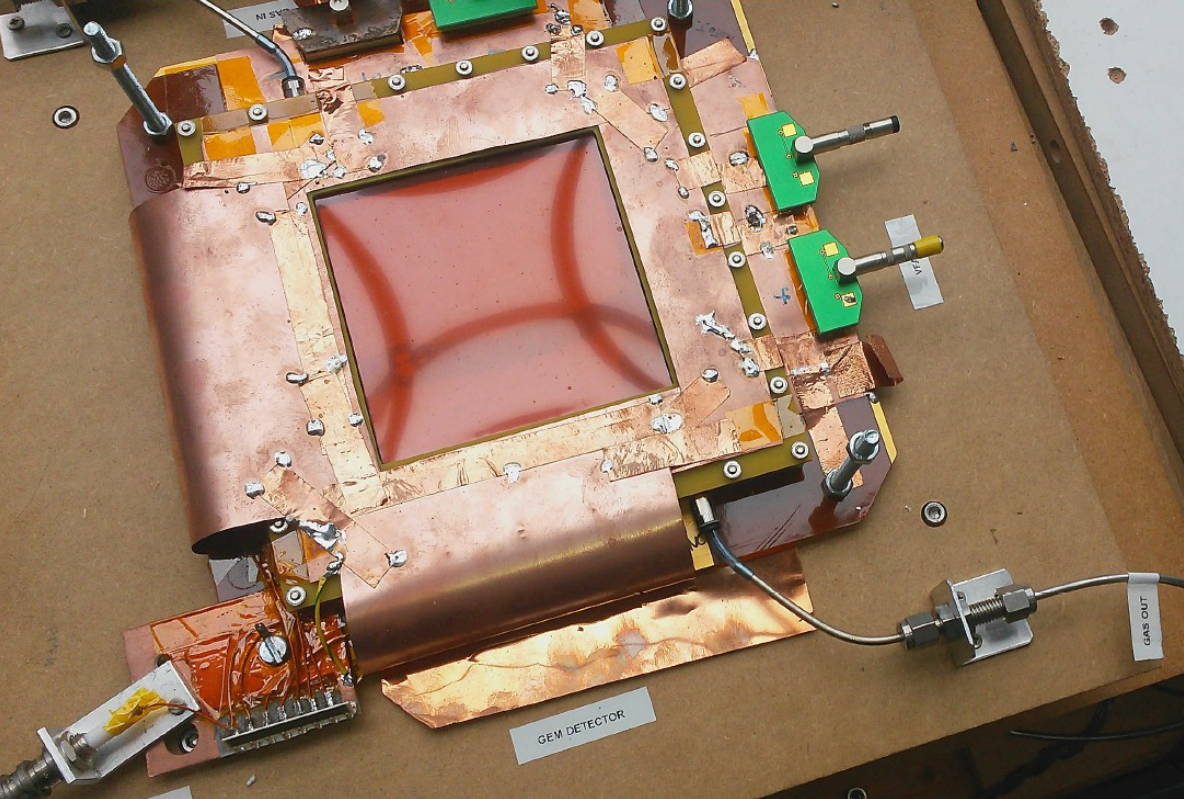
\includegraphics[width=0.8\textwidth]{img/III-1-arch/gem.png}
      \caption{}
      \label{fig:III-1-gem}
    \end{figure}

    The high voltage provided to the GEM and the photomultipliers attached to the scintillators is originating from a CAEN V6533N VME module. VME is a crate standard that defines a high speed communication protocol and an infrastructure for the interconnect of the boards. A CAEN V1718 VME-USB bridge board is used to control the communication of the VME crate from a computer. This modules allows the latter to talk to any board in the crate by initiating requests. The gas flow is regulated by four HORIBA STEC SEC-N112MGRW mass flow controllers: three for the Ar, CO$_2$, and CF$_4$ gas bottles and one to monitor the mixture. Figure \ref{fig:III-1-gas-hv} shows photographs of the VME high-voltage module on the left and the mass flow meters on the right.

    \begin{figure}[h!]
      \centering
      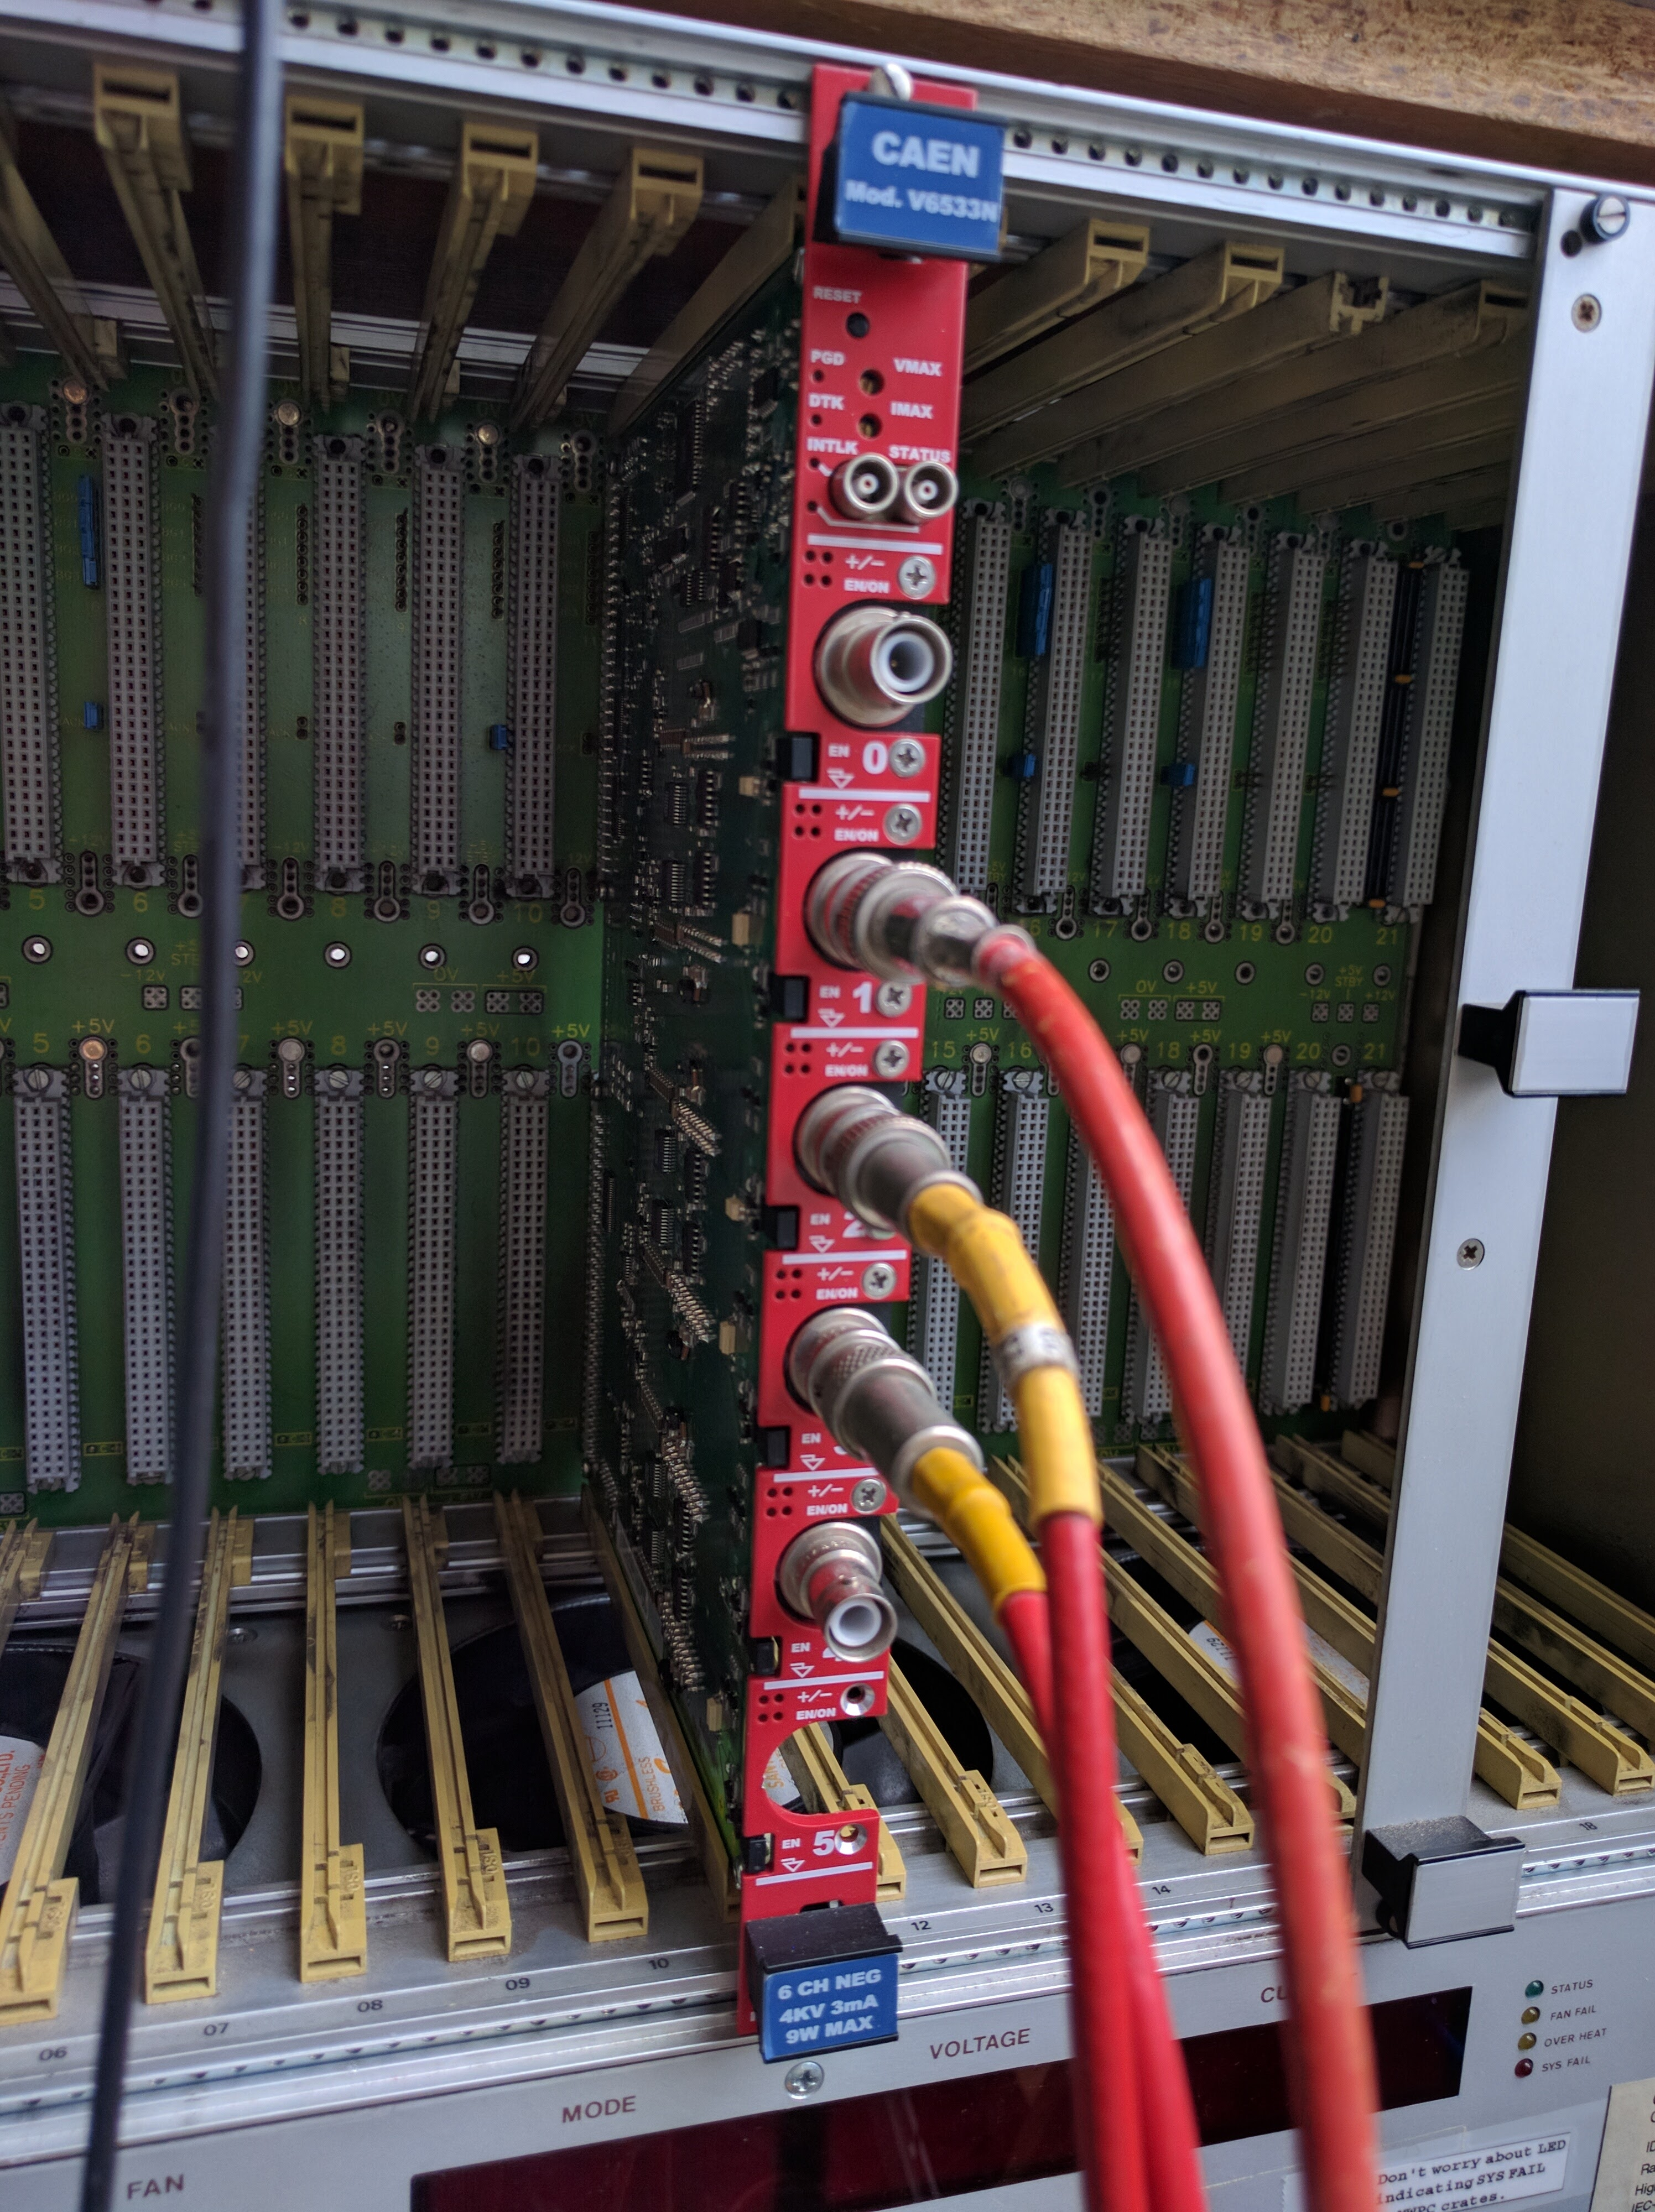
\includegraphics[width=0.39\textwidth]{img/III-1-arch/hv.jpg}
      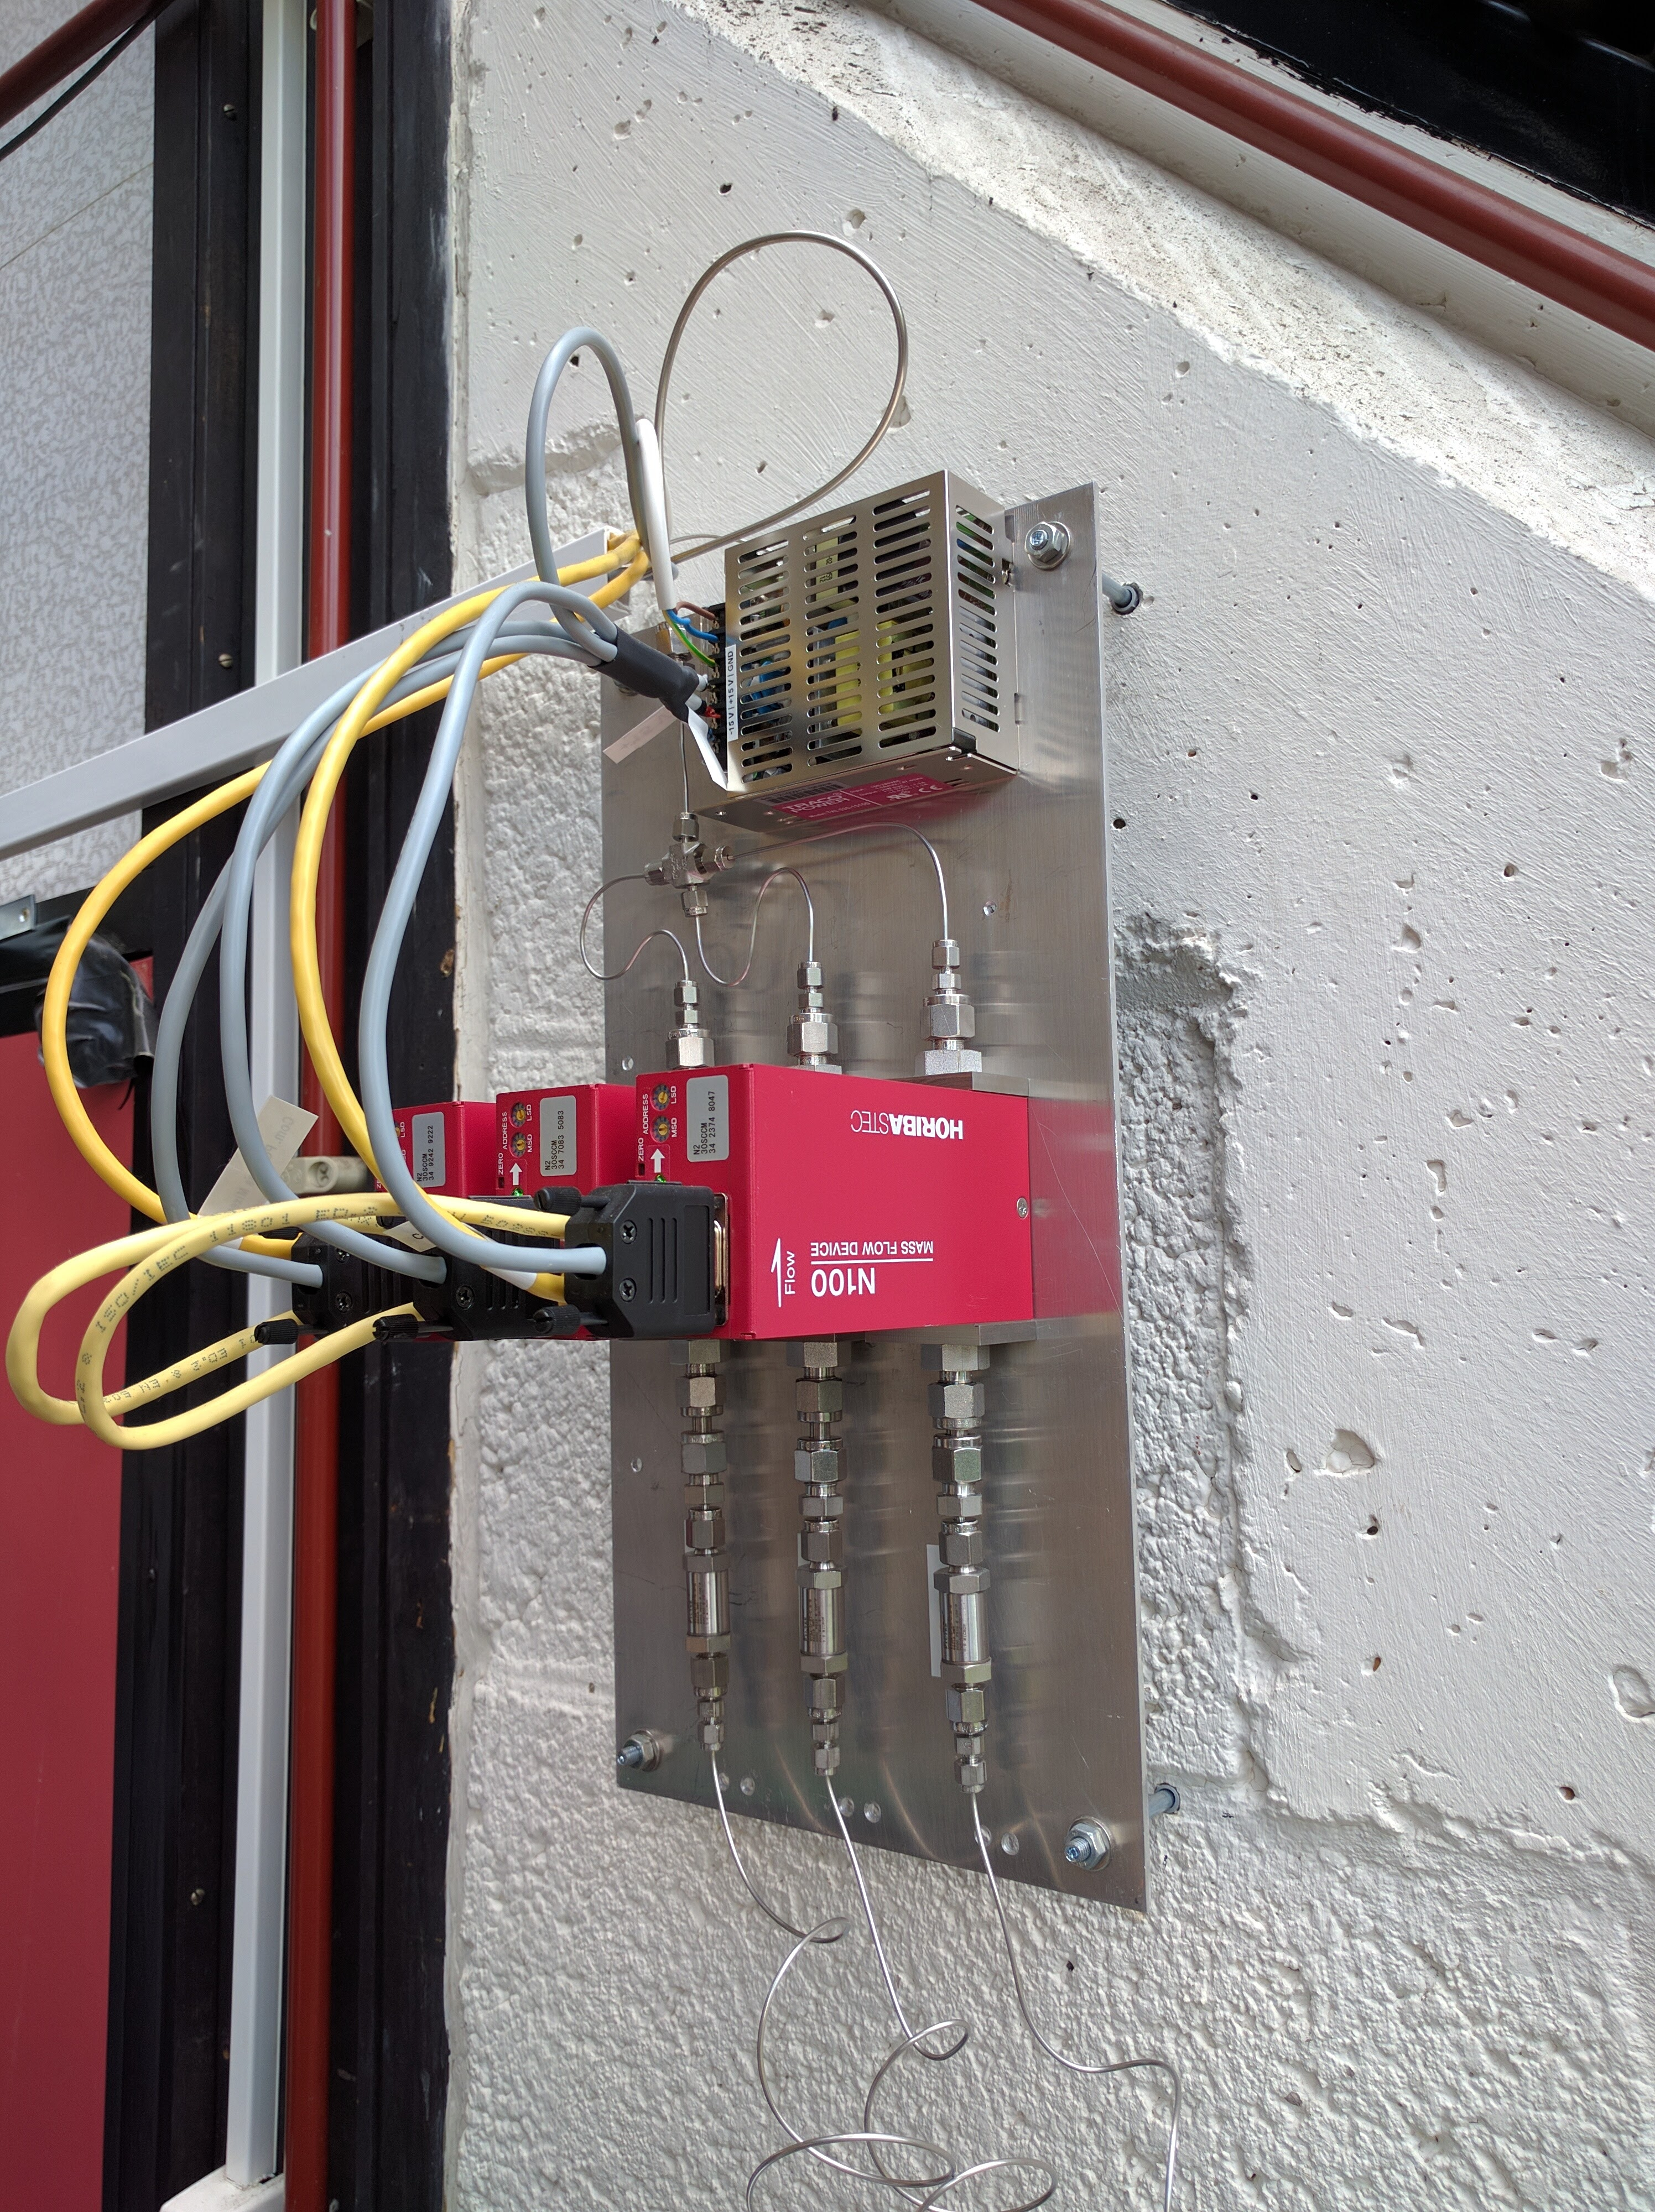
\includegraphics[width=0.39\textwidth]{img/III-1-arch/gas.jpg}
      \caption{}
      \label{fig:III-1-gas-hv}
    \end{figure}

  \section{The Infrastructure of the System}

    To control and monitor the GEM detectors, high voltage, and gas systems, a custom solution was developed around a web interface. The latter allows the user to change parameters of the runs, visualize the evolution of the settings, access logs, etc. All this information is stored in a database located on the central computing node which also hosts the web server. The database is the communication interface between all elements. It stores requests, responses, statuses, etc. From the database, a second computer located near the experimental setup extracts the parameters that need to be set on the high voltage and gas system and handles the communication protocol with these two components. This infrastructure remained unchanged while the data readout of the GEMs evolved with time.

    \subsection{The Web Interface}

      Controlling and monitoring the elements of the system is done through a web interface which makes heavy use of JavaScript. The web server runs on NodeJS, which allows JavaScript to be executed on the back-end, and communicates with the client through Socket.IO, an implementation of the WebSocket technology which provides real-time messaging. The rendering of the page is done using Bootstrap for the design and AngularJS for the data handling. Using these technologies, the web interface provides a responsive and user friendly application. \\

      The application is divided in three areas: the run control, high voltage monitoring, and gas monitoring. The run control is where parameters of the system are set when starting a new run. The system is constantly in run status even when the voltages are off or the gas disconnected. In order to differentiate data taking runs from stand-by runs, a logbook can be accessed to retrieve the parameters of the system. \\

      To monitor the parameters during a run, the user has to use home page to access a summary of the run, or the high voltage and gas pages for more details. These list the current status of the registers and monitoring valus which can be plotted. Figure \ref{fig:III-1-app} is a list of screenshots from the web application with the home page on the top left, run page on the top right, high voltage page on the bottom left, and gas page on the bottom right. Each page defines alarms that will modify the layout of the interface if error occurs, such as incorrect values stored in the system, over heating, etc. \\

      Every action taken or value read is respectively stored or read from the database. The web interface is the link between the user and the latter.

      \begin{figure}[h!]
        \centering
        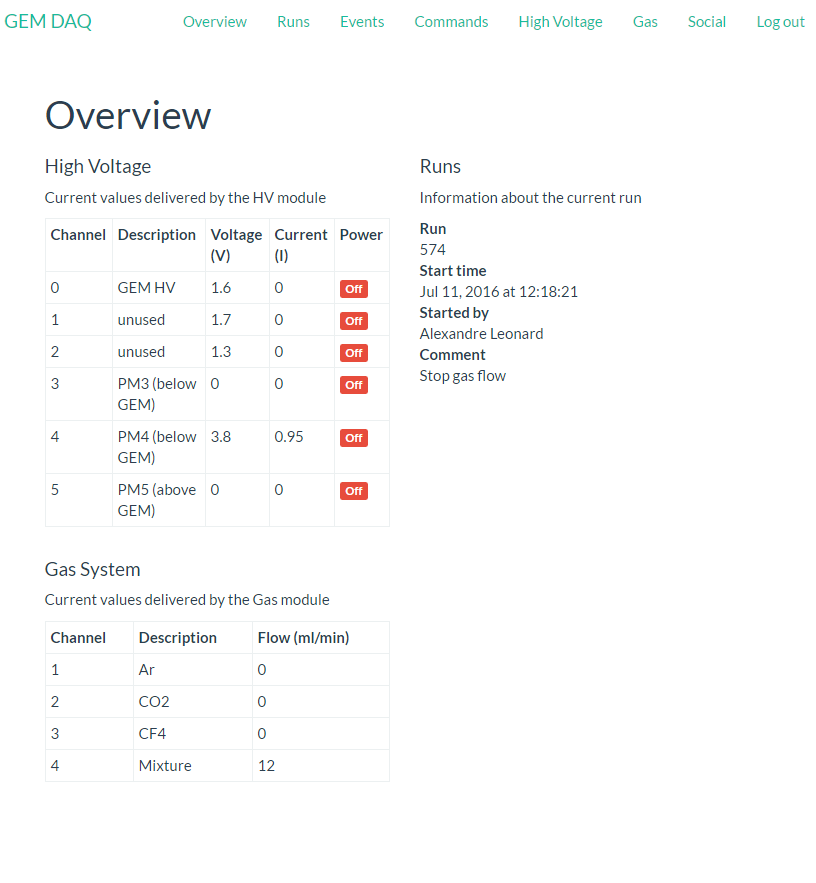
\includegraphics[width=0.49\textwidth]{img/III-1-arch/app-home.png}
        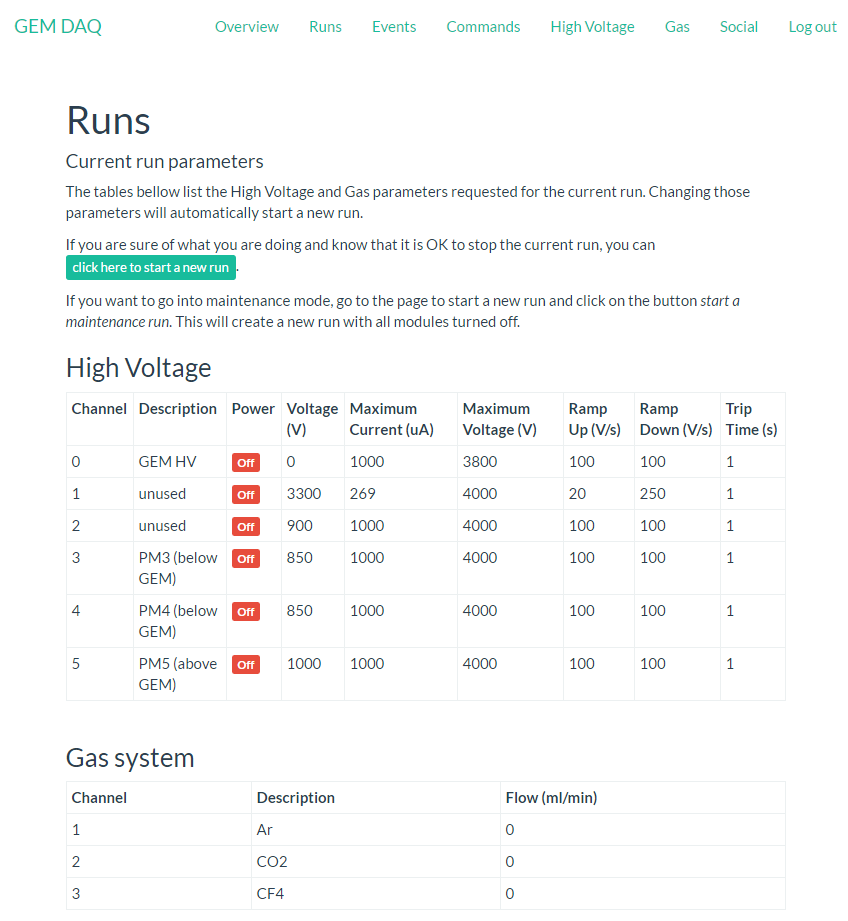
\includegraphics[width=0.49\textwidth]{img/III-1-arch/app-runs.png} \\
        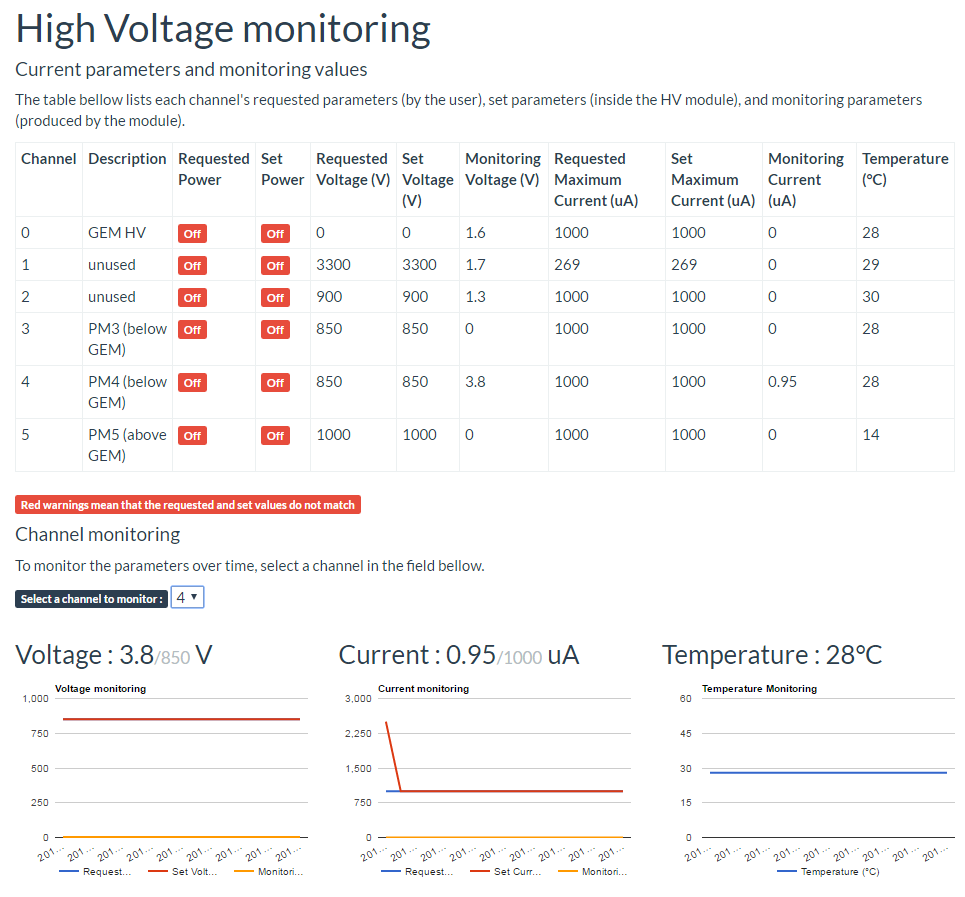
\includegraphics[width=0.49\textwidth]{img/III-1-arch/app-hv.png}
        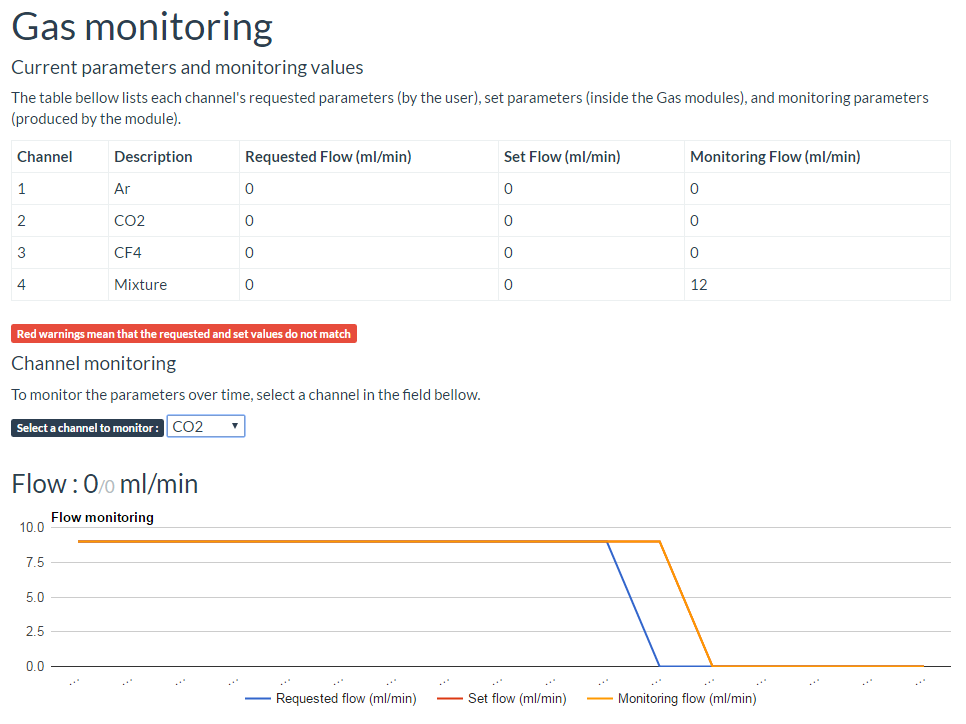
\includegraphics[width=0.49\textwidth]{img/III-1-arch/app-gas.png}
        \caption{}
        \label{fig:III-1-app}
      \end{figure}

    \subsection{The Central Computing Node}

      The central computing node is located in a server rack far from the experimental setup. It holds the web server and the MySQL database. its main role is to log every action and store the monitoring data. It is the bottleneck of the system which limits communication throughput as it has to operate various operations on the database for each request which are relatively slow.

    \subsection{The High Voltage and Gas Controller}

      The communication between the database and the high voltage and gas systems is done through a computer placed in a rack near the experimental setup. Custom software was developped by the ULB DAQ team to communicate with the VME crate and the mass flow controllers. CAEN provides an integrated library to perform read/write operations on the crate which is used to apply the parameters stored in the database. Communication with the flow meters is done through UART in the same application. 

  \section{A First Prototype using the Xilinx SP601 Development Board}

    \section{The MicroBlaze Softcore Processor}

    \section{IPBus over UART}

  \section{Upgrade of the System using the GLIB}

  \section{Final System using the First Prototype of the OptoHybrid}

























  \section{Conclusion}
